Como se mencionaba en el capitulo anterior, cada acoplamiento es
evaluado a través de una función evaluadora. El detalle es que esta
fase de evaluación se ha convertido en todo un reto para los
científicos computacionales por la dificultad de decidir de forma
determinística si un acoplamiento es bueno o no. Esto se traduce en
que la pose que se evalua como la ``mejor'' está realmente alejada de
la pose cristalográfica, y la pose más cercana a la cristalográfica
esta mucho más abajo en el ranking de poses ``buenas'' dada por esta
evaluación.

En este trabajo se propone un acercamiento con una red neuronal
convolucional para hacer un meta-análisis de dichos acoplamientos,
comparando las poses cristalográficas con las dadas por el acoplamiento
simulado.

\section{Preparación de la base de datos}
La base de datos de la cual partimos es la de el Banco de Datos de
Proteínas (PDB, \textit{Protein Data Bank}), que proporciona acceso a
resultados de estudios estructurales de macromoléculas
biológicas\footnote{\url{https://www.rcsb.org/}}. Este banco está
compuesto poralrededor de 150,000 moléculas tridimensionales
determinadas experimentalmente a las que se tiene libre acceso. El
formato utilizado para almacenar esta información (.pdb) contiene
elementos como coordenadas de átomos, nombres de moléculas e
información sobre estructuras primarias y secundarias. Es con este
formato con el que se trabajó durante el proyecto.

Inicialmente, se descargaron todas las proteínas alojadas en el banco
y se fue haciendo un filtrado de ellas del siguiente modo:
\begin{enumerate}
  \item Nos interesa estudiar acoplamientos, entonces se trabaja únicamente
  con proteínas que contuvieran ligandos. El resto queda descartado.
  \item Se eliminan todas las proteínas que tuvieran un peso
    molecular menor a 300Da. Debajo de este valor se encuentran
    principalmente iones y moléculas de bufer de cristalización.
  \item Se quitan de las proteínas las moléculas solventes
  como DMSO, PEG y MES, los cuales no son de relevancia biológica.\@
  \item Se filtran de las proteínas las cadenas de ADN o ARN.\@
  \item Se quitan también todos los metales pesados de las proteínas.
  \item Finalmente, se transforma el archivo .pdb en un archivo .pdbqt.
  Esto quiere decir que se definen las cargas de la proteína así como
  sus libertades de torsión (a las que más adelante
  llamaremos \textit{ramas}). Para esto se utilizó el programa
  MGLTools\footnote{\url{http://mgltools.scripps.edu/}}
\end{enumerate}

\begin{figure}[H]
  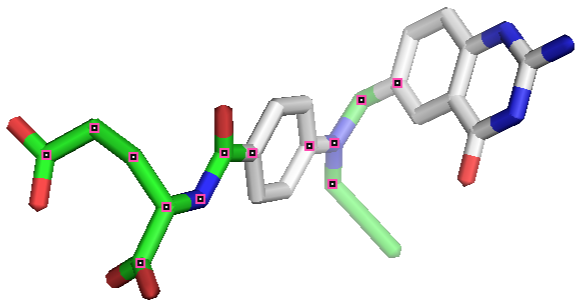
\includegraphics[scale=0.45]{torsions} \centering
  \caption{Ligando CB3 con sus ejes de torsión marcados en rosa.}
\end{figure}

Después, se hace la separación en cada proteína entre ligando y
receptor, y para cada pareja se realiza un acoplamiento virtual
utilizando \textbf{AutoDock Vina
  1.1.2}\footnote{\url{http://vina.scripps.edu/index.html}}, teniendo
así una base de datos de 24,964 acoplamientos.  Esto genera un listado
de poses, donde cada pose es un archivo .pdbqt, junto con una
calificación asociada, dada por la función evaluadora de AutoDock
Vina, de qué tan ``buena'' es la pose dada.  Con esto, se hace una
tabulación de cada pose y su calificación contra el RMSD a la pose
cristalográfica original. Esta tabla sirve como entrada para
\textit{Deep-pose}.

\begin{figure}[]
  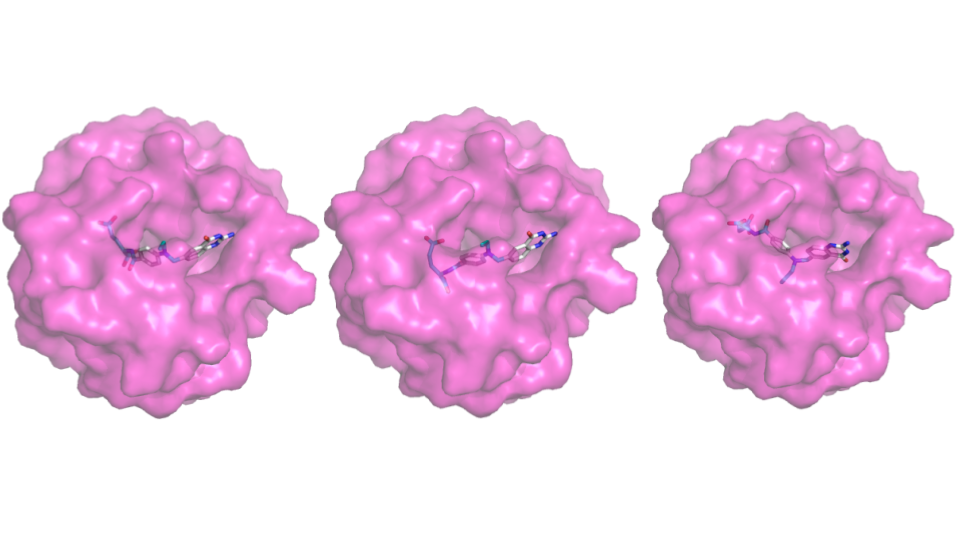
\includegraphics[scale=0.45, left]{poses}
  \caption{Primeras tres poses de acoplamiento del ligando CB3
    con el receptor 4EIL.}
\end{figure}

\begin{table}[H]
\begin{tabular}{|c|c|c|c|}
\hline
Pose         & \begin{tabular}[c]{@{}c@{}}Clasificación\\ (según AutoDock Vina)\end{tabular} & Calificación & RMSD  \\ \hline
4EIL\_CB3\_A & 1                                                                             & 10.22        & -10.2  \\
4EIL\_CB3\_A & 2                                                                             & 9.86         & -10.0  \\
4EIL\_CB3\_A & 3                                                                             & 9.65         & -9.8  \\
4EIL\_CB3\_A & 4                                                                             & 2.56         & -9.5  \\
4EIL\_CB3\_A & 5                                                                             & 9.84         & -9.3  \\ \hline
\end{tabular}
\caption{Extracto de la tabulación de poses contra RMSD a
la información cristalográfica. El formato de nombre de las poses
es \{compuesto\}\_\{ligando acoplado\}\_\{cadena\}.}
\label{tab:poses}
\end{table}

\section{Deep-pose}
\textbf{Deep-pose} es una red neuronal convolucional profunda que toma
la información de la pose de un acoplamiento en un complejo
proteína-ligando como entrada y produce una calificación de qué tan
viable es dicha pose.  Primero, dada una entrada de un complejo
proteína-ligando $x$, se extrae información del contexto local de cada
rama. El \textit{contexto} de una rama está dado por información
estructural básica (\textit{tipo de rama} y distancia). Después, cada
una de estas características básicas de cada rama es convertida en
vectores característicos que utiliza la red para aprender. Luego, una
capa convolucional es empleada para sintetizar la información de todos
los contextos de todas las ramas del ligando y generar una
representación vectorial del complejo. Posteriormente se pasa a una
capa oculta para síntesis y procesamiento del
vector-ligando. Finalmente, en la última capa, la representación del
complejo es dada como entrada a un clasificador \textit{softmax}, que
es responsable de producir el puntaje.

A continuación se presenta un pseudo-código de alto nivel del proceso
de la red:
\newpage
\begin{algorithm}[H]
  \caption{Deep-pose}
  \begin{algorithmic}[1]
    \State \textbf{Entrada:} complejo proteína-ligando x,
    donde el ligando tiene $n$ \textit{ramas}
    \State \textbf{Dados:}\newline
                           $W^{b\_type} \in \mathbb{R}^{N\times |B|}, W^{b\_dist}
                           \in \mathbb{R}^{N\times |B|},\newline
                           W^{conv} \in \mathbb{R}^{|z_i| \times cf}, W^3 \in
                           \mathbb{R}^{cf \times h},\newline
                           W_{out} \in \mathbb{R}^{h \times 2},\newline
                           b^{conv} \in \mathbb{R}^{cf}, b^{3} \in
                           \mathbb{R}^{h},\newline
                           b^{out} \in \mathbb{R}^{2}$
    \State $Z \gets [..]$
    \For{$i\gets 1, n$}
      \State $z_{b\_type} \gets$ columnas de $W_{b\_type}$
      correspondientes a los tipos de ramas de los vecinos de la
      rama $i$
      \State $z_{b\_dist} \gets$  columnas de $W_{b\_dist}$
      correspondientes a las distancias de los vecinos de la rama $i$
      \State $z_i \gets \{z_{b\_type}, z_{b\_dist}$\}
      \State $Z.add(z_i)$
    \EndFor
    \State // $U$ es inicializada con ceros
    \State $U \gets [..] \in \mathbb{R}^{cf \times n}$
    \State // Capa convolucional
    \For{$i\gets1, n$}
      \State $U[:,i]\gets f(W^{conv}Z[i] + b^{conv})$
    \EndFor
    \State // \textit{max-pooling} por columnas
    \State $r\gets \max(U, axis=1)$
    \State //Capas oculta y de salida
    \State $score\gets W^{out}(W^3r + b^3) + b^{out}$
    \State // Regresa el puntaje normalizado
    \State \textbf{return} $\frac{e^{score[1]}}{e^{score[0]}+e^{score[1]}}$
  \end{algorithmic}
\end{algorithm}
Veamos a detalle cada una de las partes de la red.

\subsection{Contexto de la rama}
Pereira, Caffaren y dos Santos \cite{dossantos} consideran al átomo
como una entidad ligada íntimamente a su contexto. Bajo esta premisa,
crean una red que toma como entrada a cada átomo del ligando con su
contexto codificado, entendiendo contexto del átomo como las
carácteristicas de éste y de los átomos más cercanos.  Pereira,
Caffaren y dos Santos buscaban encontrar valores de acoplamiento que
correspondieran con la eventual medición de la energía de enlace, sin
importar cual fuera la conformación necesaria para poder realizarlo.
Nuestro enfoque busca dar preferencia a la identificación de poses
que correspondan con una eventual pose cristalográfica.

Partiendo de la idea del átomo ligado a su contexto, y considerando
que lo que buscamos es una propiedad puramente estructural, tomamos
como unidad básica del ligando a los segmentos con libertad
rotacional, a la que llamaremos \textit{rama}. Así, nuestro
\textit{contexto de átomo} se convierte en \textbf{contexto de rama},
siendo éste la combinación del tipo de rama, los de las ramas más
cercanas y la distancia a cada una de ellas.

\subsection{Codificación del contexto de la rama}
SMILES (\textit{Simple Molecular Input Line Entry System}) es un
sencillo lenguaje químico que permite describir moléculas y reacciones
utilizando únicamente caracteres ASCII\footnote{El American Standard
  Code for Information Interchange es un estándar de codificación de
  caracteres para la comunicación informática.} que representan
símbolos de átomos y enlaces. Una cadena SMILES contiene la misma
información que una tabla de conexiones extendida, pero con varias
ventajas: es sumamente compacta y puede ser canonizada de tal manera
que puede ser usada como identificador universal para una estructura
química dada.\footnote{\url{http://www.daylight.com/smiles/}}

Se divide cada receptor y ligando en sus respectivas ramas y cada una
de estas ramas se codifica usando la respresentación SMILES. Esta
codificación, representa de forma única a cada rama distinta; es a
esto a lo que llamamos \textbf{tipo de rama}. Se enlistan todos los
tipos de rama, asociando a cada uno un índice, generando así lo que
llamamos el \textit{diccionario de ramas}.

IMAGEN HISTOGRAMA DE DISTRIBUCIÖN DE TIPOS DE RAMA

Del mismo modo, se segmentan los rangos de distancia encontrados en
compartimentos, y a cada uno de estos se les asigna también un índice,
generando así un \textit{diccionario de distancias}.

\begin{table}[H]
  \begin{center}
    \begin{tabular}{l|l}
      SMILES                 & Idx \\ \hline
      NC1=N{[}C{]}(=NC=C1)=O & 93 \\
      C1CCCCC1               & 94 \\
      CNC=O                  & 95 \\
      NC=N                   & 96 \\
      CC=C                   & 97
    \end{tabular}
    \begin{tabular}{l|l}
      Rango de distancia (\AA) & Idx \\ \hline
      3.0526 - 3.2631        & 6   \\
      3.2632 - 3.4736        & 7   \\
      3.4737 - 3.6842        & 8   \\
      3.6843 - 3.8947        & 9   \\
      3.8948 - 4.1052        & 10
    \end{tabular}
  \end{center}
  \caption{Fragmento de los diccionarios de ramas y de distancias}
  \label{fig:dictionary}
\end{table}

A partir de estos diccionarios, se asocia a una rama del ligando con
las cinco ramas del receptor más cercanas codificadas a través de sus
tipos y sus distancias a las ramas dadas. Lo que se genera entonces es
un vector con dos tuplas, donde cada elemento de las tuplas son
índices de tipos de rama y distancia respectivamente; a este vector le
llamamos el \textit{vector de rama}. El conjunto de vectores de rama
de un ligando genera la \textit{matriz de ligando}, que será la
entrada de la red.

\begin{table}[H]
  \begin{center}
  \begin{tabular}{l|l}
    OP(O)O & \AA \\ \hline N & 5.794664 \\ C1CC1 & 5.691862
    \\ NC1=N{[}C{]}(=NC=C1)=O & 4.449922 \\ NC=N & 3.785496 \\ O &
    3.747894
  \end{tabular}
  \end{center}
  \begin{equation*}
  \downarrow
  \end{equation*}
  \begin{equation*}
    OP(O)O=\begin{bmatrix}
    (2, 13, 93, 96, 4) & (4, 2, 2, 6, 4)
    \end{bmatrix}
  \end{equation*}
  \caption{Traducción de una rama a su representación vectorial}
\end{table}

Tanto para los tipos de rama, como para las particiones de distancia, se
generan las matrices $W^{b\_type}$ y $W^{b\_dist}$ respectivamente. Estas
matrices constituyen los pesos de la primera capa de la red y son
inicializadas con valores aleatorios.

\subsection{Representación vectorial del contexto de rama}

La primera capa de la red toma cada matriz de ligando y la transforma
en una matriz en $\mathbb{R}$. Cada columna en $W^{b\_type} \in
\mathbb{R}^{N\times |B|}$ corresponde al vector característico de un
tipos de rama, donde $B$ es el conjunto de tipo de ramas y $N$ es la
dimensión de los vectores característicos, quedando como un
hiperparámetro a definir.  Dado el contexto de una rama, la red
transforma cada tipo de rama en su respectivo vector característico,
utilizando los índices ya generados, y luego concatena los vectores
para generar la representación vectorial del tipo de rama
$z_{b\_type}$. Analogamente, se genera el vector $z_{b\_dist}$ en el
contexto de la rama objetivo.

\begin{table}[H]
  \begin{equation*}
    Rama=\begin{bmatrix}
    OP=O, & OC=O, & C=O, & OPO, & OP=O
    \end{bmatrix}
  \end{equation*}
  \begin{center}
    $W_{b\_type}=$
    \begin{tabular}{|l|l|l|l|l|l|l|}
      \hline
      \rowcolor[HTML]{D0D0D0}
      OP=O & OC=O & OPO & C=O & NC=O & OPO & OP=O \\ \hline
      &      &     &     &      &     &      \\ \hline
      &      &     &     &      &     &      \\ \hline
      &      &     &     &      &     &      \\ \hline
    \end{tabular}
  \end{center}
  \begin{equation*}
  \downarrow
  \end{equation*}
  \begin{equation*}
    z_{b\_type}^T =
  \begin{tabular}{lllllllllllllll}
\multicolumn{3}{l}{OP=O}                                               &                       & \multicolumn{3}{l}{OC=O}                                              &                       & \multicolumn{3}{l}{C=O}                                               &                       & \multicolumn{3}{l}{OPO}                                               \\ \cline{1-3} \cline{5-7} \cline{9-11} \cline{13-15}
\multicolumn{1}{|l|}{} & \multicolumn{1}{l|}{} & \multicolumn{1}{l|}{} & \multicolumn{1}{l|}{$\bullet$} & \multicolumn{1}{l|}{} & \multicolumn{1}{l|}{} & \multicolumn{1}{l|}{} & \multicolumn{1}{l|}{$\bullet$} & \multicolumn{1}{l|}{} & \multicolumn{1}{l|}{} & \multicolumn{1}{l|}{} & \multicolumn{1}{l|}{$\bullet$} & \multicolumn{1}{l|}{} & \multicolumn{1}{l|}{} & \multicolumn{1}{l|}{} \\ \cline{1-3} \cline{5-7} \cline{9-11} \cline{13-15}
  \end{tabular}
  \end{equation*}
  \caption{Representación de la construcción del tipo de rama ($z_{b\_type}$).
    El símbolo $\bullet$ representa la operación de concatenación.}
\label{my-label}
\end{table}

Finalmente, la representación del contexto de la rama $b$ se define
como $z_b = z_{b\_type} \cdot z_{b\_dist}$. El objetivo es que, a
partir de características básicas contextuales, la red pueda aprender
a distinguir rasgos abtractos de las ramas que permitan la
discriminación entre poses válidas y señuelos.

\subsection{Representación de la pose de un complejo proteína-ligando}

La segunda capa en la red es una capa convolucional encargada de
extraer más características abstractas de las representaciones de los
contextos de ramas y sintetizar la información de todas ellas en un
vector $r$ de longitud fija.

El problema esencial que resuelve el uso de una capa convolucional es
la capacidad de manejar entradas de distintas dimensiones. Dado que la
cantidad de ramas por ligando es variable, el uso de una capa
convolucional posibilita el procesamiento de complejos de distintos
tamaños.

Dado un complejo $x$ conformado por $n$ ramas, la entrada de la capa
convolucional es una lista de vectores $\{z_1, z_2, ..., z_n\}$ donde
$z_i$ es la representación vectorial del contexto de la $i$-ésima rama
del ligando. En la primera etapa de la capa, la extracción de
características más abstractas de cada vector $z_i$ está dada por
\begin{equation}
  u_i = f(W^{conv}_{z_i} + b^{conv})
\end{equation}
donde $W^{conv} \in \mathbb{R}^{cf \times h_1}$ es la matriz de pesos
correspondiente a la capa convolucional, $b^{conv}$ es el sesgo, $f$
es la función tangente hiperbólica y $u_i \in \mathbb{R}^{cf}$. El
número de unidades o filtros ($cf$) en la capa convolucional es un
hiperparámetro definido por el usuario.

La segunda etapa en la capa convolucional correspondiente a la etapa
de agrupación (\textit{pooling} en inglés) se encarga de sintetizar
las características de los contextos de rama. La entrada consiste en
un conjunto de vectores $\{u_1, u_2, ..., u_n\}$. Utilizamos una capa
de \textit{max-pooling} que produce un vector $r \in \mathbb{R}^{cf}$,
donde el valor del $j$-ésimo elemento está definido como el máximo de
los $j$-ésimos elementos del conjunto de vectores de entrada:
\begin{equation}
  [r]_j = \max_{1 \leq i \leq n} [u_i]_j
\end{equation}
El vector resultante $r$ de esta etapa es la representación de la pose
del complejo proteína-ligando. De este modo, la red puede aprender a
generar una representación vectorial que sintetice la información del
complejo que sea relevante para discriminar poses válidas de señuelos.

\subsection{Calificación de la pose}
El vector $r$ es procesado por dos capas neuronales básicas más: una
tercera capa oculta que representa un nivel más de abstracción y una
cuarta y última capa de salida, que computa una calificación para cada
una de las posibles clasificaciones de la pose: (0) pose señuelo y (1)
pose válida. Formalmente, dada la representación $r$ de la pose del
complejo x, la capa oculta y la de salida se computan de la siguiente
manera:
\begin{equation}
  s(x) = W^{out}(w^3r + b^3) + b^{out}
\end{equation}
donde $W^3 \in \mathbb{R}^{hxcf}$ es la matriz de pesos de la tercera
capa oculta, $W^{out} \in \mathbb{R}^{2xh}$ es la matriz de pesos de la
capa de salida, y $b^3 \in \mathbb{R}^h$ y $b^{out} \in \mathbb{R}^2$ son
sesgos. El número de unidades en la capa oculta, $h$, es un hiperparámetro
que está definido por el usuario. $s(x) \in \mathbb{R}^2$ es un vector
que contiene las calificaciones de cada una de las dos clases.

Sean $s(x)_0$ y $s(x)_1$ las calificaciones de las clases 0 y 1,
respectivamente, transformamos estas calificaciones en una
distribución de probabilidad utilizando la función \textit{softmax}:
\begin{equation}
  p(0|x) = \frac{e^{s(x)_0}}{e^{s(x)_0}+e^{s(x)_1}}
\end{equation}
\begin{equation}
  p(1|x) = \frac{e^{s(x)_1}}{e^{s(x)_0}+e^{s(x)_1}}
\end{equation}
donde decimos que $p(0|x)$ y $p(1|x)$ es la probabilidad condicional
de que la pose del compuesto sea válida o sea señuelo,
respectivamente, dados los datos obtenidos a partir del acoplamiento
del complejo proteína-ligando.

\subsection{Entrenamiento de la red}
\textit{Deep-pose} se entrenó utilizando un algoritmo de
\textbf{descenso estocástico por el gradiente}
(SGD, \textit{Stochastic Gradient Descent}).
En este caso, SGD se utiliza para minimizar la función de costos sobre
un conjunto de entrenamiento $D$ que contiene poses tanto válidas como
señuelos. En cada iteración, un nuevo complejo $(x,y) \in D$ es
elegido al azar, donde $y=1$ si la pose es válida y $y=0$ en caso
contrario. Después la red, junto con los parámetros $\theta
= \{W^{b_{type}}, W^{b_{dist}}, W^{conv}, W^3, W^{out}, b^{conv},
b^{3}, b^{out}\}$ es utilizada para estimar la probabilidad
$p(y|x, \theta)$. Finalmente, el error en la predicción se computa
como la probabilidad logarítmica negativa, $-\log(p(y|x, \theta))$, y
los parámetros de $\theta$ son actualizados
utilizando retropropagación.
\begin{equation}
  \theta \longmapsto \sum_{(x,y) \in D} -\log p(y|x, \theta)
\end{equation}

En este trabajo, se utilizaron \textit{minilotes} de complejos, 20 por
lote, y tomamos el promedio del error de la predicción para realizar
la retropropagación. La red se implementó utilizando la biblioteca
Theano.\footnote{http://deeplearning.net/software/theano/}
